\documentclass[11pt]{article}
\usepackage[margin=1in]{geometry}
\usepackage{graphicx}
\usepackage{booktabs}
\usepackage{amsmath}
\usepackage{siunitx}
\usepackage[round]{natbib}
\usepackage[hidelinks]{hyperref}
\usepackage{caption}
\usepackage{placeins}
\captionsetup{font=small, labelfont=bf}

\title{Correcting AIFS Tropical Cyclone Intensity Forecasts:\\
Reproduction, Tail-Aware Learning, and a Probabilistic Extension}
\author{Michel Faloughi\\ \small SCMP 5990 Independent Study, University of Pennsylvania}
\date{October 2026 (draft)}

\begin{document}
\maketitle

\begin{abstract}
AI weather models such as ECMWF's AIFS-Single forecast tropical cyclone tracks well but
systematically underestimate intensity, because a $0.25^{\circ}$ grid cannot resolve the eyewall.
\citet{allen2026aifstc} showed that a simple machine-learned correction, trained on tabular features
of the forecast itself, removes most of this bias. This report reproduces the gradient-boosted half
of that work at reduced scale, using only public data: 399 operational AIFS-Single forecasts
covering every North Atlantic and East Pacific storm from February 2025 to September 2026, tracked
with a purpose-built MSLP-minimum tracker and corrected with gradient-boosted trees under
storm-grouped cross-validation. The raw model's maximum-wind mean absolute error (MAE) of
30.3\,kt is more than halved to 14.4\,kt, against 9.4\,kt for the official NHC forecast.
Raw-model error and the rapid-intensification failure mode match the paper almost exactly
(71.4\,kt vs.\ their 71.1\,kt raw MAE on RI cases), while the corrected error remains above the
paper's 11.0\,kt, consistent with training on one and a half seasons instead of nine years.
The tracker is validated against ECMWF's own operational AIFS tracks to within 1.1\,kt MAE.
The second half of the report asks whether a learned correction can be made to respect the
observed tail of the intensity distribution, and what that buys. Eta-learning
\citep{chang2026eta}, a tail-matching penalty on a small neural network, beats a tuned MSE network
by 1.1\,kt overall (95\% storm-bootstrap CI $[-2.3, -0.03]$) and by 5.6\,kt on rapid
intensification (RI) cases, and beats the classical post-hoc quantile-mapping baseline by 2.1\,kt;
most of its advantage over an untuned network, however, is regularization. A diagnosis of
\emph{which} storms receive the extreme forecasts shows the penalty controls how many extreme
forecasts are issued, not where they go, a limitation shared by any point forecast forced to match
the observed marginal. The constructive response is a probabilistic correction: quantile
gradient boosting with a cross-conformal recalibration step gives 80\% intervals that cover
82\% of out-of-storm cases and 84\% of a future season, and a median that is 0.8\,kt better than
the point GBM in cross-validation. Adding SHIPS-type environmental predictors computed from the
AIFS pressure-level fields helps by about 1\,kt at short leads and not at all on RI, and the
derived probability of RI has no skill over climatology with 15 RI storms of training data.
\end{abstract}

\section{Introduction}

Data-driven weather models have reached operational skill for synoptic-scale prediction, and
ECMWF's AIFS-Single \citep{lang2024aifs} runs operationally alongside the physics-based IFS. For
tropical cyclones these models inherit a structural weakness: with grid spacing of about 28\,km,
the inner core of a hurricane is unresolved, so forecast 10\,m winds saturate far below observed
intensity even when the track is accurate. \citet{allen2026aifstc} (``AIFS-TC'') demonstrated that
this bias is largely \emph{predictable}: a gradient-boosted model over simple features of the AIFS
forecast and the operationally known initial intensity brings AIFS intensity forecasts to parity
with the operational frontier.

This project asks how much of that result survives a drastic reduction in resources: public data
only, one and a half hurricane seasons instead of nine years of hindcasts, a home-made tracker, and
a laptop. Beyond the replication itself, the by-product is an end-to-end open pipeline (catalog,
fetch, track, correct, evaluate) of roughly 900 lines of Python.

The reproduction exposes the weakness that motivates the rest of the report: the corrected
forecasts never reach the observed extremes. Trees cannot extrapolate beyond their training
targets, so the GBM never forecasts above about 125\,kt while nine storms in the sample reached
120\,kt or more. Sections~\ref{sec:eta} to \ref{sec:prob} study three responses in turn: a
tail-matching training objective (eta-learning), richer inputs (environmental predictors of the
kind used by the operational SHIPS scheme), and a probabilistic output with calibrated intervals.
Every comparison is reported as a paired difference with a storm-level bootstrap interval, because
the effective sample is the number of storms (52), not the number of cases (9149).

\section{Data}

\paragraph{AIFS forecasts.} The ECMWF Open Data AWS mirror (\texttt{s3://ecmwf-forecasts},
CC-BY-4.0) retains every operational AIFS-Single run since 2025-02-25. Storm lifetimes from the
IBTrACS best-track archive \citep{knapp2010ibtracs} define 399 forecast initializations (00/12
UTC) covering all North Atlantic (NA) and East Pacific (EP) storms of at least tropical-storm
strength through 2026-09-08. For each run, only the GRIB messages for mean sea-level pressure and
10\,m winds are downloaded via HTTP byte ranges, cropped to $0$--$60^{\circ}$N,
$180^{\circ}$W--$0^{\circ}$, at leads 0--168\,h every 6\,h (7.1\,GB total, versus hundreds of GB
for the full archive).

\paragraph{Reduction caveats.} The stored arrays are a lossy reduction: three surface variables,
one basin pair, leads capped at 168\,h (the mirror holds 360\,h), and winds stored in half
precision (error well below $0.1$\,kt, negligible against forecast error).

\paragraph{Pressure-level fields for environmental predictors.} For Section~\ref{sec:ships}, ten
further fields were pulled for every run and lead from the same archive (via its Google Cloud
mirror, which does not rate-limit byte-range requests): $u$ and $v$ at 850 and 200\,hPa,
temperature at 200, 500 and 700\,hPa, specific humidity at 500 and 700\,hPa, and skin
temperature. Cropped to the same box this adds 23\,GB. The tabular dataset used from
Section~\ref{sec:eta} onward is the full set of 9149 labelled (storm, initialization, lead)
cases from 52 storms, which is larger than the homogeneous sample of Section~\ref{sec:results}
because it does not require an OFCL forecast to exist at the same lead.

\paragraph{Operational archive, not hindcasts.} Unlike the paper's controlled hindcast training
set, these are the forecasts actually issued in real time. Two consequences matter. First, the
model version changes mid-dataset: AIFS-Single 1.0 was operational for the 2025 season and 2.0
(released 2026-05-12) for 2026; a version flag is passed to the correction model and results are
reported by season. Second, each run starts from the real-time operational analysis with its
data-assimilation cutoff, not from a reanalysis.

\paragraph{Verification and benchmarks.} Ground truth is the IBTrACS/ATCF best track (USA agency
values). The benchmark is OFCL, the official human forecast of the National Hurricane Center,
parsed from the ATCF a-deck archive, which also supplies GDMN, the ensemble mean of Google
DeepMind's cyclone model \citep{deepmind2025weatherlab}, and EAIO, ECMWF's own tracker applied to
the same AIFS runs.

\section{Methods}

\paragraph{Tracker.} Each forecast is seeded at the best-track position at initialization. At each
6\,h step the storm is located at the MSLP minimum within 450\,km of a first guess (previous
position advected with previous motion) on a lightly smoothed field; intensity is that minimum
pressure and the maximum 10\,m wind within 250\,km. Tracking stops when the low is no longer
distinct. Against ECMWF's operational AIFS tracks (EAIO) at matched initialization and lead
($n=1209$, 24 storms), the tracker agrees to a mean difference of $+0.8$\,kt and an MAE of
1.1\,kt, so tracker choice is not a meaningful error source.

\paragraph{Correction model.} Following the GBM branch of AIFS-TC, gradient-boosted trees
(scikit-learn \texttt{HistGradientBoostingRegressor}, 5-seed average) predict the residual between
best-track and AIFS maximum wind. The 22 features include the AIFS forecast state and its trends
and running extremes, translation speed, basin, day of year, the model-version flag, storm age,
the observed intensity and 12/24\,h intensity trend at initialization, and the initial AIFS bias.
Observed rapid-intensification cases (RI, $\ge 30$\,kt observed gain in 24\,h) are weighted
$2\times$ in training, as in the paper. Evaluation uses storm-grouped 5-fold cross-validation, so
a storm is never corrected by a model that saw any part of it. A persistence-of-initial-bias
baseline (carrying the initialization-time AIFS bias forward unchanged) is included as a sanity
check; the GBM beats it at every lead beyond 24\,h.

\section{Results of the reproduction}\label{sec:results}

Table~\ref{tab:main} and Figure~\ref{fig:mae} give the headline result on the homogeneous sample
(cases where raw, corrected, and OFCL forecasts all exist and verify against best track):
the correction cuts overall MAE from 30.3 to 14.4\,kt, with non-overlapping 95\% confidence
intervals from a storm-level bootstrap. It does not reach OFCL (9.4\,kt) overall, but approaches
it at long leads (16.4 vs.\ 14.1\,kt at 120\,h). On a separate homogeneous sample containing
GDMN ($n=2022$, 41 storms), DeepMind's dedicated cyclone model scores 9.9\,kt, on par with OFCL
(9.6), with corrected AIFS at 14.6.

\begin{table}[t]
\centering
\caption{Maximum-wind MAE (kt) versus best track by forecast lead time, homogeneous sample
($n=2223$ cases, 46 storms, NA+EP, Feb 2025--Sep 2026). Bottom row: all leads pooled, with 95\%
storm-bootstrap confidence intervals.}
\label{tab:main}
\begin{tabular}{rrccc}
\toprule
Lead (h) & $n$ & AIFS raw & AIFS+GBM & NHC OFCL \\
\midrule
 12 & 442 & 26.4 & 10.8 &  4.9 \\
 24 & 396 & 28.4 & 13.2 &  7.4 \\
 36 & 358 & 29.8 & 14.9 &  9.5 \\
 48 & 315 & 31.4 & 16.3 & 10.9 \\
 72 & 247 & 33.4 & 16.6 & 11.5 \\
 96 & 190 & 35.2 & 16.7 & 12.8 \\
120 & 148 & 35.8 & 16.4 & 14.1 \\
144 &  74 & 31.7 & 16.3 & 13.6 \\
168 &  53 & 25.0 & 14.2 & 11.1 \\
\midrule
12--168 & 2223 & 30.3 [24.5, 35.1] & 14.4 [12.4, 16.6] & 9.4 [8.0, 10.5] \\
\bottomrule
\end{tabular}
\end{table}

\begin{figure}[t]
\centering
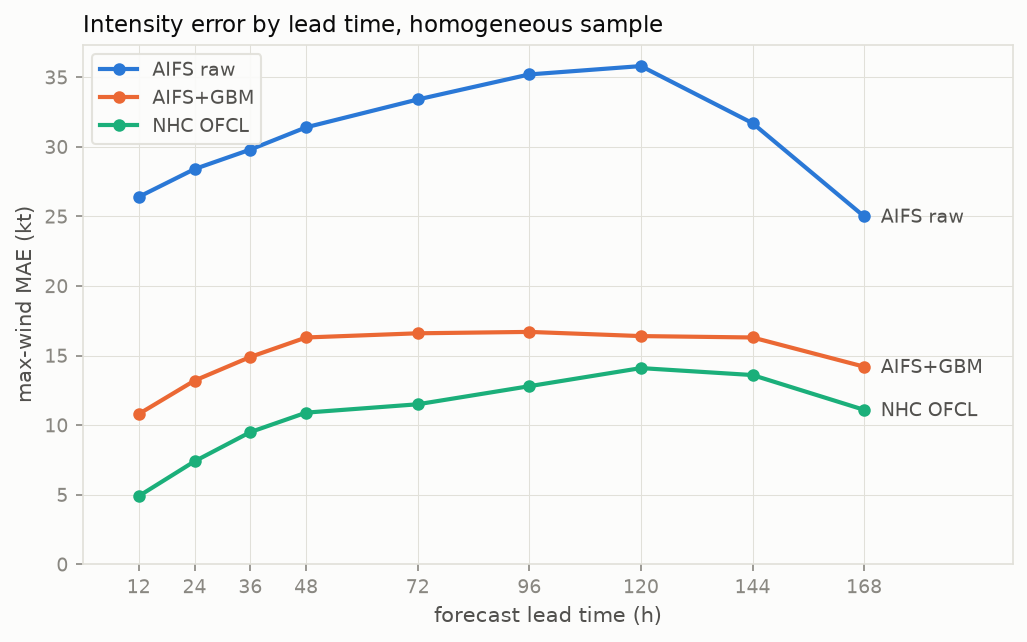
\includegraphics[width=0.85\linewidth]{figures/tc_mae_by_lead.png}
\caption{Maximum-wind MAE by lead time on the homogeneous sample. The raw AIFS error is
dominated by the under-resolution bias; the GBM correction removes most of it at every lead.}
\label{fig:mae}
\end{figure}

Table~\ref{tab:subsets} breaks the pooled result down. The correction helps in both basins and
both seasons. Notably, it performs better on the 2026 season (AIFS-Single 2.0, 12.1\,kt) than on
2025 (v1.0, 15.5\,kt) despite 2026 contributing less training data, suggesting the newer model's
errors are more systematic and therefore easier to learn. Rapid intensification remains the hard
case: raw AIFS misses RI by 71.4\,kt on average, the correction recovers roughly half of that
(38.3\,kt), and the human forecast (20.2\,kt) stays well ahead.

\begin{table}[t]
\centering
\caption{Pooled (12--168\,h) maximum-wind MAE (kt) with 95\% storm-bootstrap confidence
intervals, by subset.}
\label{tab:subsets}
\begin{tabular}{lrrccc}
\toprule
Subset & $n$ & Storms & AIFS raw & AIFS+GBM & NHC OFCL \\
\midrule
All cases          & 2223 & 46 & 30.3 [24.5, 35.1] & 14.4 [12.4, 16.6] &  9.4 [8.0, 10.5] \\
RI cases only      &  162 & 13 & 71.4 [61.7, 77.5] & 38.3 [32.0, 42.8] & 20.2 [16.5, 23.5] \\
North Atlantic     &  772 & 15 & 32.4 [22.0, 39.3] & 15.5 [10.7, 19.7] & 10.4 [7.7, 12.4] \\
East Pacific       & 1451 & 31 & 29.2 [22.2, 35.7] & 13.9 [11.4, 16.2] &  8.9 [7.4, 10.2] \\
2025 (AIFS 1.0)    & 1526 & 30 & 29.6 [23.2, 35.5] & 15.5 [12.9, 18.1] &  9.6 [8.2, 10.9] \\
2026 (AIFS 2.0)    &  697 & 16 & 31.8 [20.1, 39.2] & 12.1 [8.4, 14.5]  &  8.8 [5.8, 10.9] \\
\bottomrule
\end{tabular}
\end{table}

Figure~\ref{fig:lowell} shows the raw bias at its most dramatic: Hurricane Lowell (EP, 2026)
reached 140\,kt while every raw AIFS forecast saturated near 60\,kt. Figure~\ref{fig:map} shows
the underlying fields and tracks for one initialization with three simultaneous storms.

\begin{figure}[t]
\centering
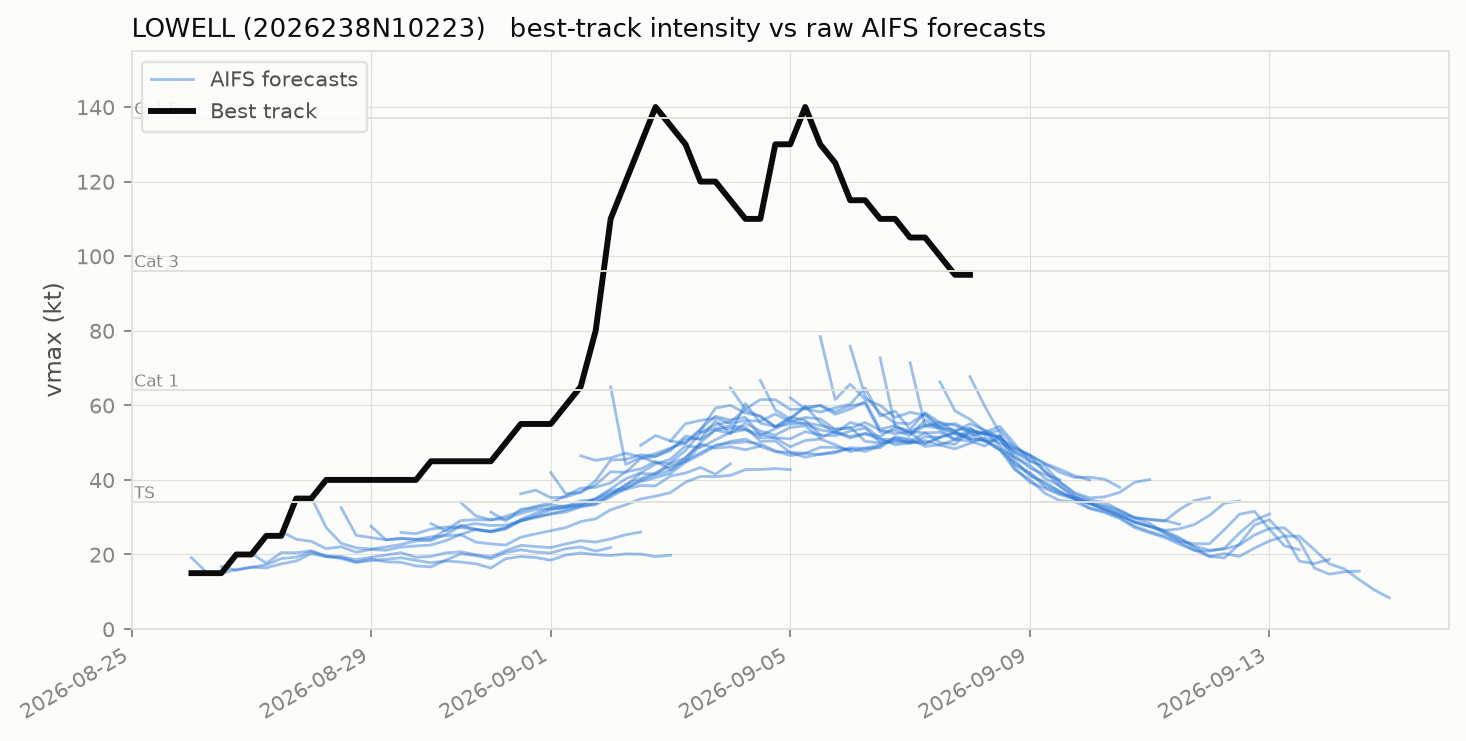
\includegraphics[width=0.9\linewidth]{figures/tc_intensity_lowell.png}
\caption{Observed intensity of Hurricane Lowell (2026, EP; black) against all 27 raw AIFS
forecasts (blue). The model's track is good but its intensity saturates near 60\,kt against an
observed peak of 140\,kt: the under-resolution bias the correction targets.}
\label{fig:lowell}
\end{figure}

\begin{figure}[t]
\centering
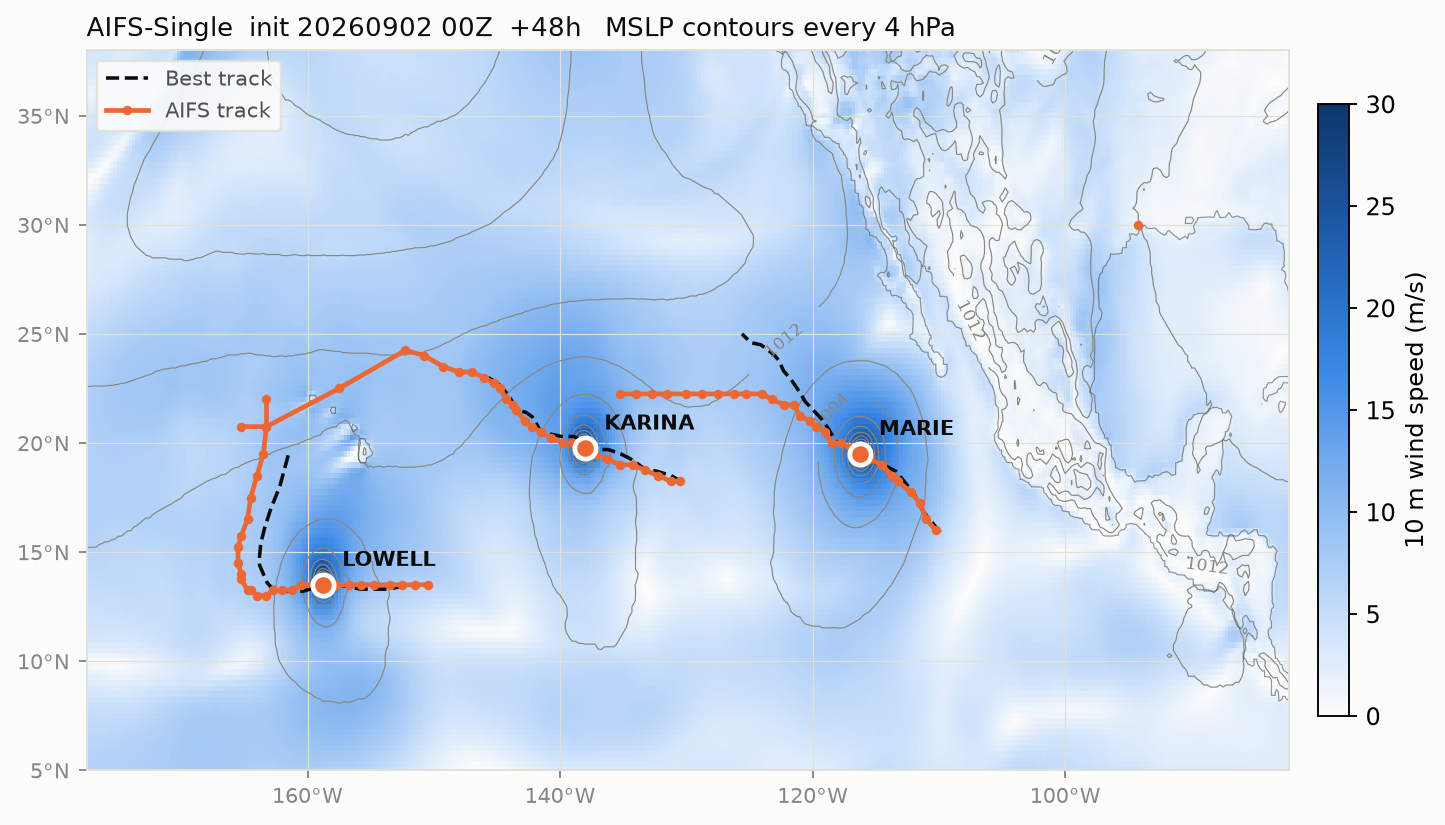
\includegraphics[width=0.95\linewidth]{figures/tc_map_2026090200_048h.png}
\caption{AIFS-Single forecast fields at $+48$\,h from the 2026-09-02 00Z run: 10\,m wind speed
(shading), MSLP (contours every 4\,hPa), forecast tracks (orange) and best tracks (dashed) for
hurricanes Lowell, Karina and Marie.}
\label{fig:map}
\end{figure}


\FloatBarrier
\section{Evaluation protocol for everything that follows}\label{sec:protocol}

Three conventions hold for Sections~\ref{sec:eta} to \ref{sec:prob}. (i) Models predict the
residual $r = v_{\mathrm{obs}} - v_{\mathrm{AIFS}}$ and are scored on the corrected wind
$v_{\mathrm{AIFS}} + \hat r$. (ii) Cross-validation is storm-grouped and five-fold; a temporal
holdout (train on 2025 initializations, test on 2026: 20 storms, 4121 cases, 222 RI cases from
4 storms) is reported where the model is cheap enough to refit. (iii) Any difference between two
models is a \emph{paired} difference, with a 95\% interval from resampling storms with
replacement 2000 times. Treating cases as independent would understate the uncertainty by a
factor of two or more: a quick check on twenty years of NHC forecasts found that nominal 95\%
intervals built on cases cover the truth 65 to 73\% of the time, while the storm bootstrap covers
95\% overall but only 86 to 93\% on extreme subsets. Every number on an extreme subset therefore
also states the number of storms behind it.

\section{Eta-learning: a tail-matching objective}\label{sec:eta}

\paragraph{Method.} \citet{chang2026eta} propose training a regressor with the usual mean-squared
error plus a penalty that pulls the upper quantiles of its \emph{predictions} toward the same
quantiles of a reference distribution $\nu_0$ of the target. Here the network is a 64-64 ReLU
multilayer perceptron on the 22 features of Section~3, trained full-batch with Adam
(learning rate $3\times10^{-3}$, 600 iterations, three seeds averaged), the penalty is the mean
absolute gap between 25 quantiles (levels 0.95 to 0.999) of the corrected wind over the training
fold and the same quantiles of the observed wind in that fold, and the weight $\lambda$ is set
every 100 iterations by the ratio of gradient norms of the two terms, as in the paper. The
plain-MSE network with the penalty switched off (``ERM'') is the natural control.

\paragraph{Ablation.} Table~\ref{tab:eta} separates the three things that differ between the
paper's GBM and the eta network: architecture, objective, and the $2\times$ RI weighting.

\begin{table}[t]
\centering
\caption{Ablation grid: MAE (kt) on all 9149 cases and on the 585 RI cases (15 storms),
storm-grouped 5-fold CV. ``$2\times$RI'' doubles the weight of RI cases in training.}
\label{tab:eta}
\begin{tabular}{llcc}
\toprule
Architecture & Objective & All & RI \\
\midrule
GBM & MSE                  & 13.8 & 40.4 \\
GBM & MSE, $2\times$RI     & 14.1 & 41.1 \\
MLP & MSE (ERM)            & 17.7 & 36.6 \\
MLP & MSE, $2\times$RI     & 16.6 & 33.4 \\
MLP & eta                  & 13.1 & 29.9 \\
MLP & eta, $2\times$RI     & 13.5 & 26.1 \\
\bottomrule
\end{tabular}
\end{table}

The clean contrast is eta against ERM on the same network: $-4.6$\,kt $[-6.8, -2.2]$. Against
the GBM the overall difference is a tie ($-0.7$\,kt $[-2.0, +0.8]$), but on RI cases eta wins by
$-10.5$\,kt $[-14.4, -5.6]$. Eta is also the only model whose forecasts reach the observed tail:
its 0.95 and 0.99 forecast quantiles are 119 and 143\,kt against 120 and 140 observed, whereas the
GBM's are 98 and 118.

\paragraph{Is it calibration or climatology?} The reference $\nu_0$ above is the 18-month
training sample itself, so the penalty can only be \emph{calibrating} the network to a
distribution it already sees. The version that imports information uses $\nu_0$ from the
IBTrACS archive since 1980 (1651 storms). The result barely moves: MAE 12.8 against 13.1,
difference $-0.3$\,kt $[-1.3, +0.8]$, and on RI $+2.3$\,kt $[-1.4, +5.9]$. Eta is doing
calibration, not importing climatology.

\paragraph{Lead time and the future season.} Eta's advantage over ERM grows with lead
($-3.7$, $-4.0$, $-4.7$, $-5.3$, $-5.8$\,kt across the bands 6--24, 30--48, 54--72, 78--120 and
126--168\,h, every interval excluding zero), contrary to the expectation that matching a point
forecast to the observed tail should hurt at long leads, where the best point forecast is less
extreme than the observations. The reason is visible in the tail itself: at 126--168\,h eta's
0.99 forecast quantile is 134\,kt against 153 observed, so the penalty is no longer binding
there. On the temporal holdout (train 2025, test 2026), which is also the transfer test the advisor
asked for since 2025 runs are AIFS-Single 1.0 and 2026 runs are 2.0, the picture is unchanged: raw 27.8\,kt,
GBM 15.8, ERM 22.4, eta 15.6; eta minus GBM $-0.2$\,kt $[-3.0, +3.5]$ overall and $-7.9$\,kt
$[-15.3, -0.5]$ on RI, the latter resting on four storms.

\subsection{The fair baseline: a tuned network plus quantile mapping}\label{sec:fair}

The ERM network above has no early stopping, and its tail overshoots (0.99 quantile 160\,kt
against 140 observed), so part of eta's gain could be regularization rather than the objective.
The fair comparison, suggested by the advisor, is (a) the same network with early stopping and
weight decay chosen on held-out training storms, and (b) that network followed by quantile
mapping of its corrected winds onto $\nu_0$, the classical marginal correction of climate science
\citep{maraun2013inflation}. If eta still wins against (b), it is doing more than matching a
histogram. All five models in Table~\ref{tab:fair} were trained in one run with identical folds
and seeds.

\begin{table}[t]
\centering
\caption{The fair baseline. MAE (kt), storm-grouped 5-fold CV, 3 seeds, 52 storms; tail
quantiles of the forecasts against 120 / 140 observed. Early stopping selects 100 to 250
iterations, confirming that the 600-iteration network overfits.}
\label{tab:fair}
\begin{tabular}{lccc}
\toprule
Model & All & RI & $q_{0.95}$ / $q_{0.99}$ \\
\midrule
Plain MLP, 600 iterations                 & 17.66 & 36.78 & 123 / 160 \\
Tuned MLP (early stopping, weight decay)  & 14.42 & 35.45 & 112 / 133 \\
Tuned MLP + quantile mapping to $\nu_0$   & 15.44 & 34.71 & 122 / 160 \\
Eta                                       & 13.29 & 29.88 & 118 / 148 \\
GBM                                       & 14.12 & 41.12 &  98 / 118 \\
\bottomrule
\end{tabular}
\end{table}

\begin{table}[t]
\centering
\caption{Paired MAE differences (kt) between the models of Table~\ref{tab:fair}, with 95\%
storm-bootstrap intervals. Negative favours the first model.}
\label{tab:fairdiff}
\begin{tabular}{lcc}
\toprule
Difference & All & RI (15 storms) \\
\midrule
Eta $-$ plain MLP                 & $-4.36$ $[-7.09, -1.76]$ & $-6.89$ $[-14.71, +2.08]$ \\
Eta $-$ tuned MLP                 & $-1.12$ $[-2.30, -0.03]$ & $-5.57$ $[-9.33, -0.95]$ \\
Eta $-$ tuned MLP + QM            & $-2.14$ $[-3.23, -0.99]$ & $-4.83$ $[-8.14, -0.62]$ \\
Tuned MLP + QM $-$ tuned MLP      & $+1.02$ $[+0.09, +2.06]$ & $-0.73$ $[-1.90, +0.83]$ \\
Eta $-$ GBM                       & $-0.83$ $[-2.18, +0.51]$ & $-11.24$ $[-15.26, -6.44]$ \\
\bottomrule
\end{tabular}
\end{table}

Three of the 4.4\,kt that eta gains over the untuned network are regularization: the tuned
network alone closes the gap to 1.1\,kt. That remaining 1.1\,kt $[-2.3, -0.03]$ and the 5.6\,kt
on RI are the real effect of the objective. Quantile mapping, the post-hoc alternative, is
\emph{worse} than the tuned network by 1.0\,kt overall: forcing a point forecast to have the
observed marginal inflates its errors on ordinary cases, the well-known inflation problem of
marginal correction. Eta beats the mapped baseline by 2.1\,kt $[-3.2, -1.0]$, so it is not
reducible to calibration after the fact. Figure~\ref{fig:fair} shows the same comparison by lead
and Figure~\ref{fig:qq} the upper tail of each model.

\begin{figure}[t]
\centering
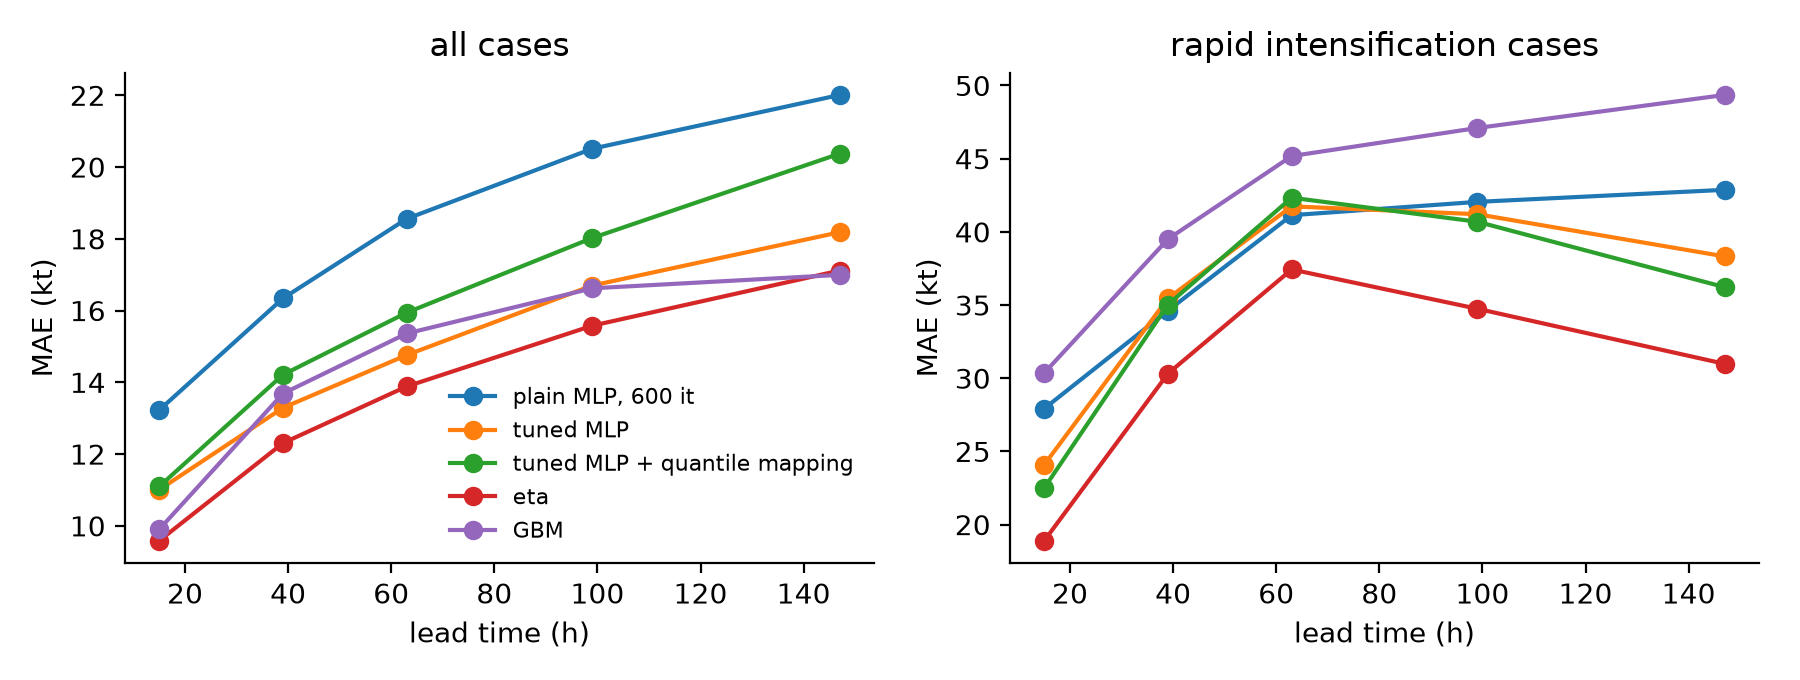
\includegraphics[width=0.95\linewidth]{figures/fair_baseline_by_lead.png}
\caption{MAE by lead time for the five models of Table~\ref{tab:fair}, all cases (left) and RI
cases (right), out-of-fold. Eta's RI advantage is present at every lead.}
\label{fig:fair}
\end{figure}

\begin{figure}[t]
\centering
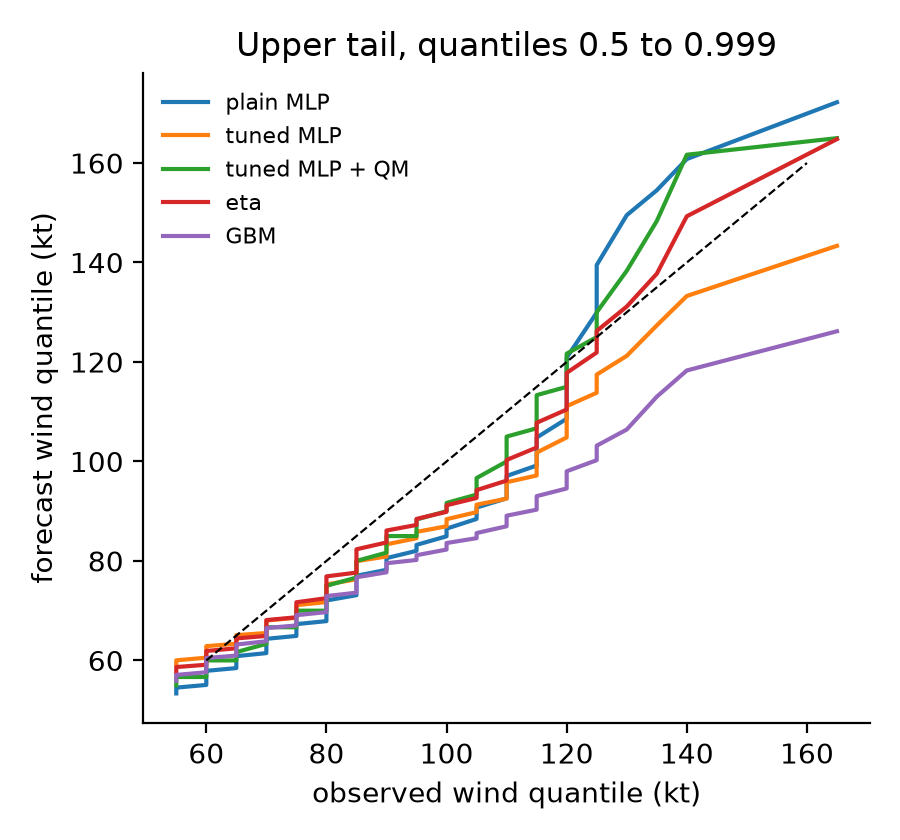
\includegraphics[width=0.5\linewidth]{figures/tail_qq.png}
\caption{Forecast against observed wind quantiles from 0.5 to 0.999, out-of-fold. The GBM stops at
125\,kt; the untuned network and the mapped network overshoot; eta follows the diagonal most
closely.}
\label{fig:qq}
\end{figure}

\FloatBarrier
\subsection{Right tails, wrong storms}\label{sec:wrongstorms}

Matching the pooled tail does not mean the extreme forecasts land on the right storms. Among
eta's 440 forecasts of 120\,kt or more, the observed wind is on average 22\,kt lower
($[-33.5, +1.7]$), and 358 of the 440 come from two storms (Lowell and Erin). Of the 636 cases
observed at 120\,kt or more, eta forecasts 120\,kt or more for 26\%. This is not specific to eta:
the untuned network overshoots by 34\,kt on its own extreme forecasts, and the GBM followed by
quantile mapping shows the same pattern ($-23$\,kt). It is the generic behaviour of a point
forecast whose marginal has been forced onto the observed one, and the eta paper states the
limitation itself (``distributionally calibrated candidate extremes, rather than \ldots\ true
location, time, or mechanism''). An attempt to fix it by applying the penalty within groups
(by initial intensity) was abandoned once the group-wise gaps were bootstrapped: every interval
includes zero. The constructive response is to stop forcing a point forecast and predict a
distribution instead (Section~\ref{sec:prob}).

\section{Environmental predictors from the forecast itself}\label{sec:ships}

The 22 features so far describe the AIFS vortex (wind, pressure, their trends) and the storm's
history, nothing about its environment. The operational SHIPS scheme
\citep{demaria1994ships, demaria2005ships} and its RI index \citep{kaplan2003ri} rest on a handful
of environmental quantities: vertical wind shear, mid-level humidity, upper-level divergence and
temperature, low-level vorticity, and the ocean's potential intensity. All of them can be
computed from the AIFS forecast's own pressure-level fields, which makes them legitimate
forecast-time features. From the fields of Section~2, each case receives: the magnitude and
direction of the ring-mean (200 to 800\,km from the forecast centre) 200 minus 850\,hPa wind
vector; relative humidity at 700 and 500\,hPa from $q$ and $T$; 200\,hPa divergence and 850\,hPa
relative vorticity within 1000\,km; 200\,hPa temperature; skin temperature within 200\,km as a
sea-surface proxy; the \citet{demaria1994ships} maximum potential intensity from it; and the
potential minus the current forecast wind. Each is taken at the forecast lead, at
initialization, and averaged along the forecast track, for 36 features in all.

Table~\ref{tab:ships} gives the effect on the point GBM. The gain is about 1\,kt, concentrated at
short leads, with intervals that touch zero, and nothing on RI. The advisor's hypothesis was that
the information bottleneck, not the objective, limits RI skill; these predictors do not lift it,
which leaves the AIFS environment at $0.25^{\circ}$, the single deterministic run, or the sample
of 15 RI storms as the remaining suspects.

\begin{table}[t]
\centering
\caption{Point GBM with and without the 36 environmental predictors. MAE (kt), storm-grouped
5-fold CV, paired storm-bootstrap intervals.}
\label{tab:ships}
\begin{tabular}{lrrccc}
\toprule
Subset & $n$ & Storms & Base & + SHIPS & Difference \\
\midrule
All cases         & 9149 & 52 & 13.99 & 13.08 & $-0.91$ $[-2.13, +0.17]$ \\
RI cases          &  585 & 15 & 40.62 & 39.60 & $-1.02$ $[-6.39, +3.67]$ \\
Lead $\le 48$\,h  & 4259 & 52 & 11.56 & 10.50 & $-1.06$ $[-2.29, 0.00]$ \\
Lead $> 96$\,h    & 2238 & 29 & 16.70 & 16.81 & $+0.11$ $[-1.93, +1.84]$ \\
\bottomrule
\end{tabular}
\end{table}

\FloatBarrier
\section{A probabilistic correction}\label{sec:prob}

\paragraph{Method.} Nine gradient-boosted regressors with the pinball loss predict the residual
quantiles at levels 0.02, 0.05, 0.10, 0.25, 0.50, 0.75, 0.90, 0.95 and 0.98 (same features as
Table~\ref{tab:ships} with SHIPS, same tree hyperparameters and RI weighting as the point GBM,
quantiles sorted to remove crossings). Quantile trees turned out to be far too confident on
unseen storms: the raw 10--90\% interval covered only 51\% of out-of-fold cases. The remedy is a
cross-conformal recalibration in the spirit of \citet{romano2019cqr} and \citet{barber2021cvplus}:
within each training fold, an inner storm-grouped 5-fold produces out-of-fold residuals
$y - \hat q_\tau(x)$ for every level $\tau$; the empirical $\tau$-quantile of those residuals,
computed separately in three lead bands (0--48, 54--96, 102--168\,h), is added to $\hat q_\tau$
at test time. Scores are the mean absolute error of the median, the continuous ranked
probability score (CRPS, approximated by twice the mean pinball loss over the nine levels
\citep{gneiting2007scoring}), and the coverage of the 10--90\% interval. The probability of RI is
read off the predicted distribution as $P(v_{t} \ge v_{t-24} + 30\,\mathrm{kt})$ and scored with
the Brier score against climatology; a direct gradient-boosted classifier on the RI label is the
baseline.

\paragraph{Calibration.} Figure~\ref{fig:calib} shows the fraction of observations falling
below each predicted quantile. The raw quantile trees are badly over-confident (10--90\% interval
covering 51\%); after recalibration the curve sits on the diagonal in cross-validation (82\%) and
on the future season (84\%), and the CRPS improves from 7.69 to 6.69\,kt. Calibration is not
uniform across cases, however: on RI cases the 80\% interval covers only 35\% in CV, and on cases
observed at 96\,kt or more it covers 51\%. The price of covering ordinary cases honestly while
being unable to tell which storms will intensify is a wide upper tail: the 0.99 quantile of the
predicted 95th percentile is 170\,kt in CV against 140 observed. The model knows it does not know.
The pooled tail of \emph{samples} drawn from the predictive distribution, which is where the
advisor suggested a tail constraint should apply, already matches the observed tail in
cross-validation without any penalty: 109, 123 and 149\,kt at levels 0.9, 0.95 and 0.99 against
110, 120 and 140 observed. The per-level recalibration achieves what the eta penalty achieves for
a point forecast, and does it on a distribution, where it is coherent. On the 2026 holdout the
sampled tail is too heavy (137 and 162\,kt at 0.95 and 0.99 against 120 and 135), because the
offsets were learned on the 2025 storms, which include the two strongest of the record.

\begin{figure}[t]
\centering
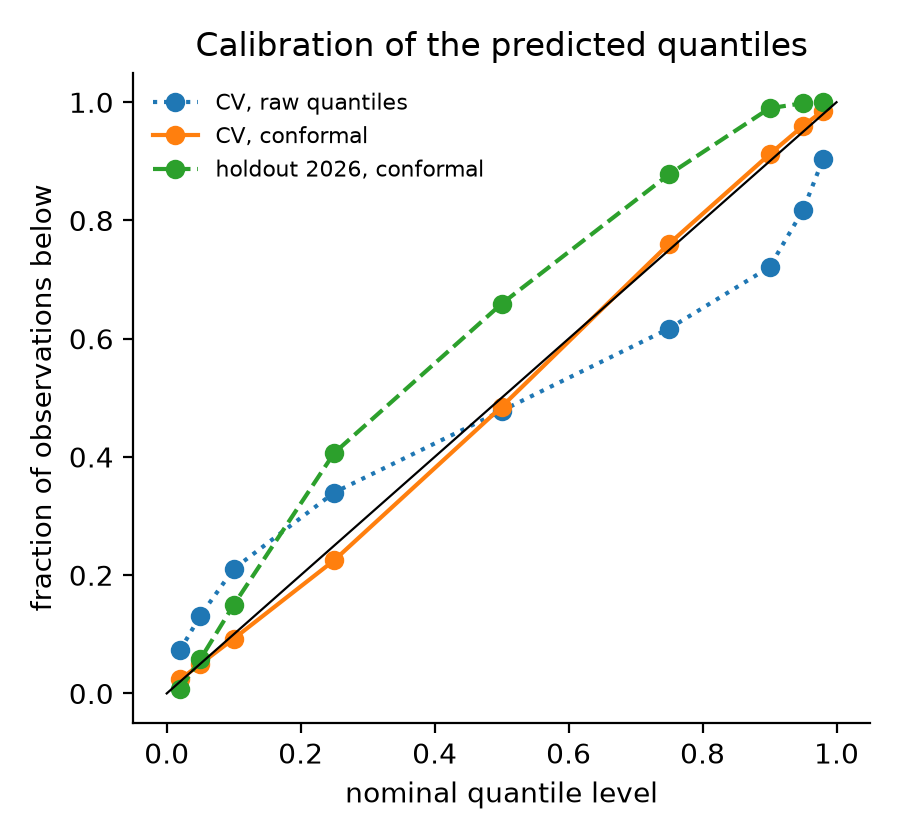
\includegraphics[width=0.48\linewidth]{figures/quantile_calibration.png}
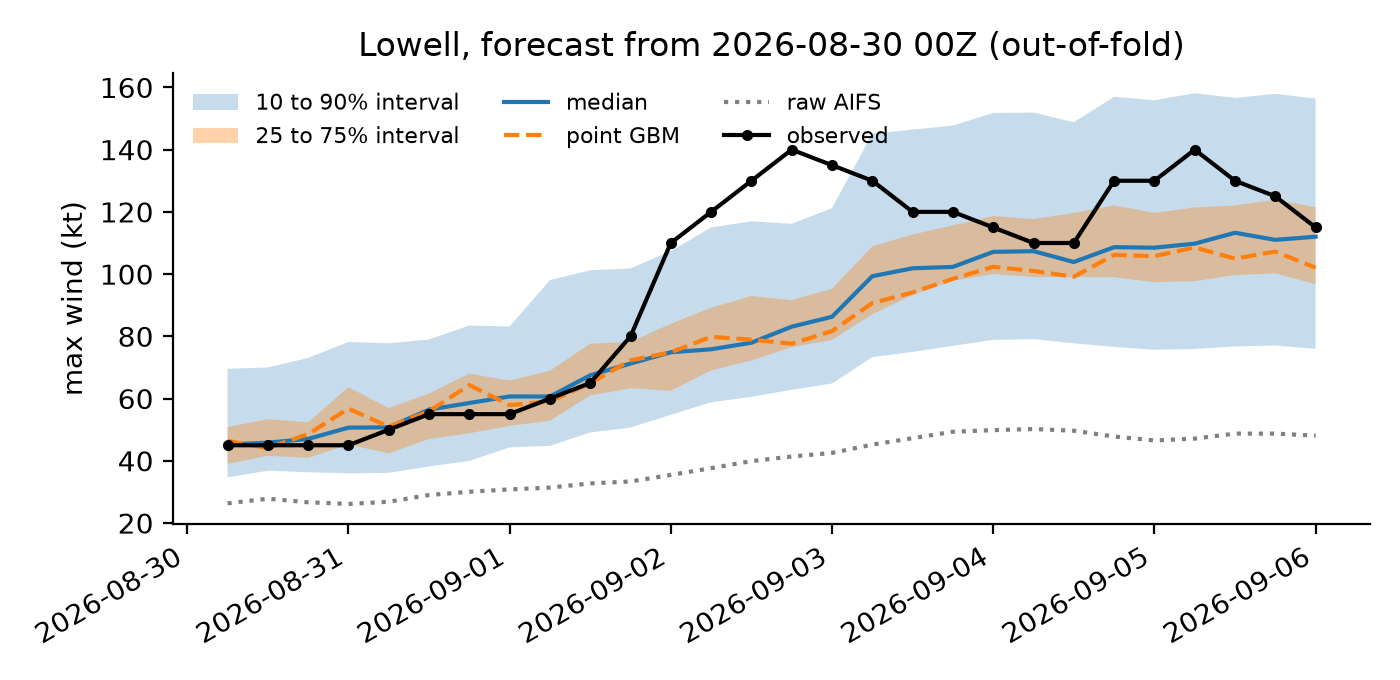
\includegraphics[width=0.5\linewidth]{figures/storm_example_lowell.png}
\caption{Left: calibration of the predicted quantiles before and after the cross-conformal step,
in cross-validation and on the 2026 holdout. Right: an out-of-fold forecast of Hurricane Lowell
(2026): raw AIFS saturates near 50\,kt, the corrected median follows the storm to about 110\,kt,
and the observed rapid intensification to 140\,kt leaves even the 10--90\% band.}
\label{fig:calib}
\end{figure}

\paragraph{Accuracy.} Table~\ref{tab:prob} compares the median of the recalibrated distribution
with the point GBM trained on the same features. In cross-validation the median is better by
$0.85$\,kt $[-1.57, -0.15]$ overall and by $2.4$\,kt $[-4.7, -0.2]$ on cases observed at 96\,kt
or more; on RI cases the difference ($-2.2$\,kt) has an interval that includes zero. On the 2026
holdout the overall difference reverses ($+0.4$\,kt $[-0.1, +1.2]$) because the median is worse
at leads of 48\,h or less, while it stays better at long leads and on strong storms. The honest
summary is that the probabilistic model costs nothing in point accuracy and adds calibrated
intervals.

\begin{table}[t]
\centering
\caption{Median of the recalibrated quantile GBM against the point GBM, same features (base plus
SHIPS). MAE (kt), paired storm-bootstrap intervals, CRPS and 10--90\% interval coverage of the
quantile model.}
\label{tab:prob}
\begin{tabular}{llrrccccc}
\toprule
Evaluation & Subset & $n$ & Storms & Median & Point & Difference & CRPS & Coverage \\
\midrule
CV      & all              & 9149 & 52 & 12.78 & 13.63 & $-0.85$ $[-1.57, -0.15]$ & 6.69 & 82\% \\
CV      & RI               &  585 & 15 & 40.66 & 42.82 & $-2.16$ $[-5.69, +0.72]$ & 18.10 & 35\% \\
CV      & lead $\le 48$\,h & 4259 & 52 & 10.28 & 10.80 & $-0.52$ $[-1.13, +0.04]$ & 5.52 & 82\% \\
CV      & lead $> 96$\,h   & 2238 & 29 & 16.36 & 17.81 & $-1.45$ $[-2.82, +0.08]$ & 8.31 & 81\% \\
CV      & obs $\ge 96$\,kt & 1444 & 13 & 33.10 & 35.49 & $-2.39$ $[-4.70, -0.19]$ & 14.99 & 51\% \\
\midrule
Holdout & all              & 4121 & 20 & 14.07 & 13.64 & $+0.43$ $[-0.14, +1.24]$ & 7.49 & 84\% \\
Holdout & RI               &  222 &  4 & 32.81 & 35.77 & $-2.95$ $[-5.72, +0.83]$ & 12.03 & 86\% \\
Holdout & lead $\le 48$\,h & 1800 & 20 & 13.58 & 12.52 & $+1.06$ $[+0.54, +1.65]$ & 6.98 & 78\% \\
Holdout & lead $> 96$\,h   & 1117 & 12 & 14.16 & 15.26 & $-1.10$ $[-2.69, +0.08]$ & 7.88 & 93\% \\
\bottomrule
\end{tabular}
\end{table}

\paragraph{Probability of rapid intensification.} This is where the project set out to arrive,
and the answer is negative. Read off the predicted distribution, $P(\mathrm{RI})$ has a Brier
skill score of $-0.06$ against climatology in cross-validation and $-0.44$ on the holdout, and
the reliability diagram (Figure~\ref{fig:rel}) shows why: when the model says 0.6, RI follows
21\% of the time in CV and 5\% on the holdout. The direct classifier on the RI label does no
better in CV ($-0.03$ with SHIPS features, $-0.05$ without), and on the holdout its score flips
sign with the feature set ($+0.08$ without SHIPS, $-0.48$ with), which with 222 RI cases from
four storms is noise. Neither the objective nor the environmental predictors turn 15 RI storms
into a usable RI probability. The failure is one of calibration more than of discrimination:
the quantile-derived probability ranks RI cases above non-RI cases with an area under the ROC
curve of 0.77 in CV and 0.72 on the holdout (the direct classifier: 0.67 and 0.70), and a warning
threshold of 0.2 catches 56\% of RI cases in CV at the cost of 81\% false alarms (76\% and 89\%
on the holdout). An isotonic recalibration of the probabilities, cross-fitted by storm, turns the
CV Brier skill positive ($+0.05$) but does not transfer to the future season ($-0.18$ when fitted
on 2025 storms only). The eta network's RI advantage of Section~\ref{sec:fair} is a gain in the
\emph{magnitude} of its forecasts on storms that did intensify, not an ability to say in advance
which storms will.

\begin{figure}[t]
\centering
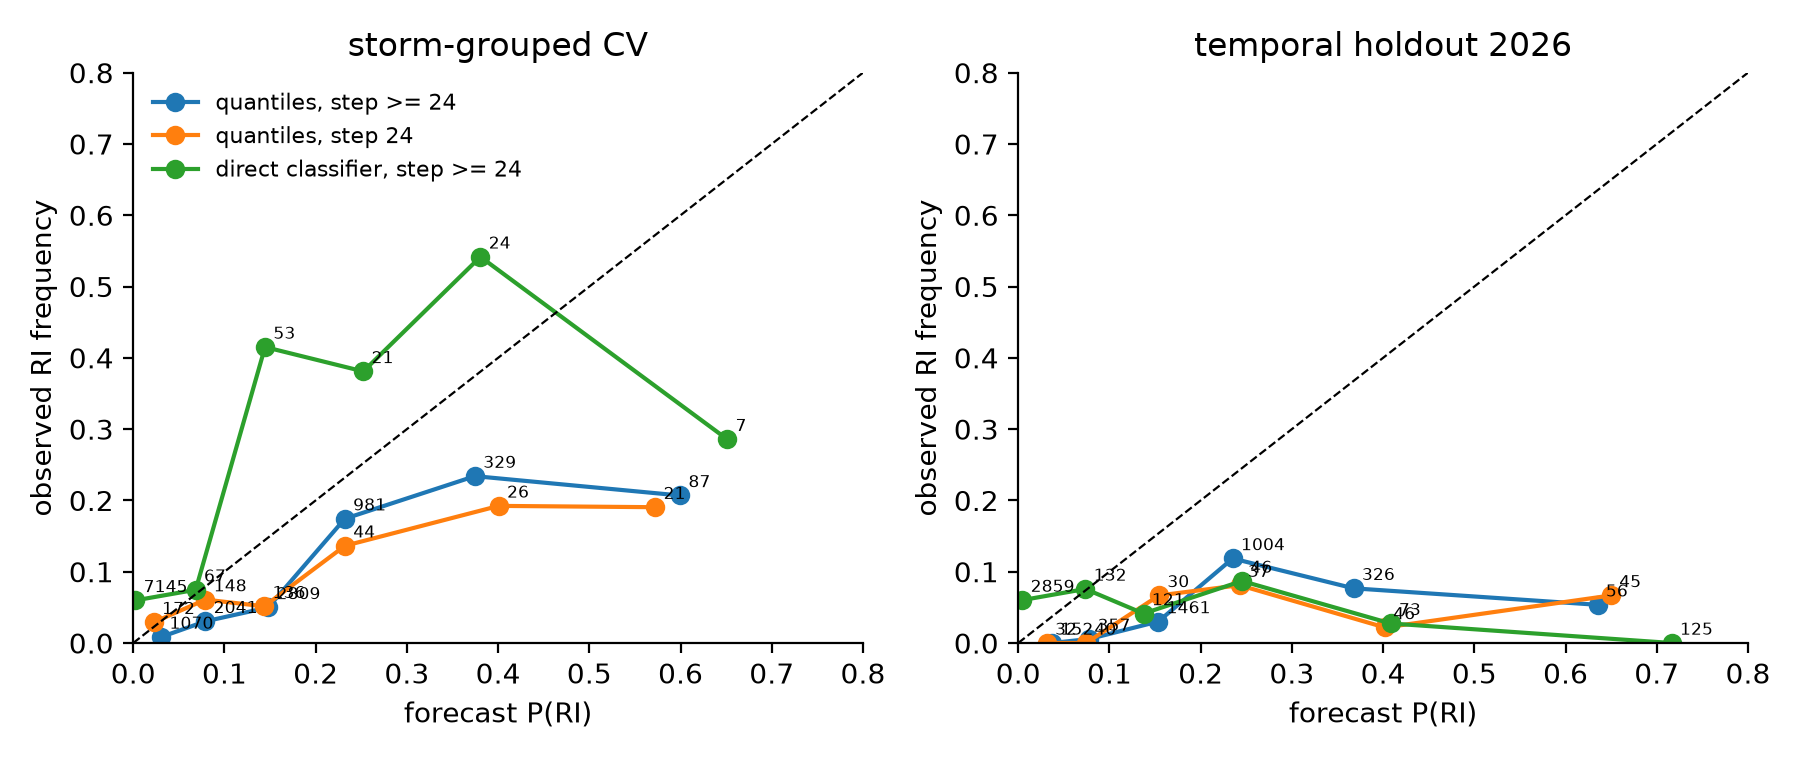
\includegraphics[width=0.95\linewidth]{figures/ri_reliability.png}
\caption{Reliability of the RI probability from the predicted distribution and from a direct
classifier, in cross-validation (left) and on the 2026 holdout (right); labels give the number of
cases in each bin. A skilful forecast would follow the diagonal.}
\label{fig:rel}
\end{figure}


\FloatBarrier
\section{What did not work}

Two further ideas were tested and dropped; both are recorded so that they are not retried.
\emph{Wind through pressure.} The observed wind-pressure relationship is tight (6.9\,kt MAE from
observed pressure), so correcting AIFS pressure and converting might beat correcting wind
directly. It does not: 15.2 against 14.0\,kt, worse by $+1.2$\,kt $[+0.1, +2.3]$, because the
correction removes 51\% of the wind error but only 13\% of the pressure error. \emph{An archive
prior.} A model of future intensity from storm history alone, trained on 45 years of IBTrACS with
no forecast input, reaches 17.6\,kt on these storms and beats the AIFS-based correction at 6--24\,h
(7.2 against 9.9). Stacked as a feature it helps when training storms are few ($-2.0$\,kt
$[-2.8, -1.1]$ with 10 storms) and not with all 41 ($-0.3$ $[-0.7, +0.2]$); a Bayesian
combination of the archive prior with an AIFS likelihood beat stacking only at 5 training storms
and was worse on RI. With a full season of paired data the archive adds nothing.

\section{Comparison with AIFS-TC}

Table~\ref{tab:paper} sets these results against the paper's NA+EP evaluation
\citep{allen2026aifstc}. The samples differ (their held-out 2025 under one model version and
hindcast initial conditions; here 2025--2026 operational output under two versions), so each
column should be read against its own OFCL, not across columns.

\begin{table}[t]
\centering
\caption{Pooled maximum-wind MAE (kt), this work versus AIFS-TC (their NA+EP test set, 29
storms). Samples differ; compare each system to its own sample's OFCL.}
\label{tab:paper}
\begin{tabular}{lcc}
\toprule
 & This work & AIFS-TC \\
\midrule
AIFS raw            & 30.3 & 35.3 \\
Corrected           & 14.4 & 11.0 \\
NHC OFCL            &  9.4 & 10.7 \\
AIFS raw, RI only   & 71.4 & 71.1 \\
Corrected, RI only  & 38.3 & 20.9 \\
OFCL, RI only       & 20.2 & 20.1 \\
\bottomrule
\end{tabular}
\end{table}

Three observations. First, the \emph{baselines} land on the paper's numbers: raw AIFS error is
the same phenomenon at the same magnitude, and on RI cases the agreement is striking (71.4 vs.\
71.1\,kt). Together with the 1.1\,kt tracker agreement, this indicates the pipeline measures the
same quantity the paper measures. Second, the \emph{correction} reproduces the qualitative claim,
recovering roughly three quarters of the raw-to-OFCL gap, but not the paper's parity with OFCL.
Third, the shortfall concentrates exactly where limited training data should hurt most: rare RI
events, of which this dataset contains 13 storms' worth against the paper's nine years. The
2026-only result (12.1\,kt, single model version) already approaches the paper's 11.0.

\section{Limitations}

One and a half seasons versus nine years of training data, and 52 storms of which 15 produced RI
and 9 reached 120\,kt: every RI or tail statistic in this report rests on a handful of storms, and
the intervals say so. Two model versions in one dataset, handled only by a feature flag. The GBM
branch of AIFS-TC only (no CNN over three-dimensional patches), and a single deterministic AIFS
run: the AIFS ensemble is in the same archive from July 2025 and its spread was not used.
Best-track initial intensity as a feature where fully operational practice would use the
real-time CARQ estimate (the paper reports both variants); two basins; leads capped at 168\,h.
Position errors are measured but not corrected. The eta network was tuned once (the paper's
settings) and the quantile model inherits the point GBM's hyperparameters; neither was searched.
Model variants for the dropped ideas of Section~\ref{sec:wrongstorms} and the archive prior were
chosen after seeing results and are reported as negative findings only.

\FloatBarrier
\section{Reproducibility}

All code is at \url{https://github.com/MichelFaloughi/scmp-5990}: the data pipeline in
\texttt{pipeline/} (catalog, fetch, track, correct, evaluate, and the pressure-level fetch and
SHIPS predictor scripts), the modeling of Sections~\ref{sec:eta} to \ref{sec:prob} in
\texttt{core/} (\texttt{gbm.py}, \texttt{eta.ipynb}, \texttt{paired\_ci.ipynb},
\texttt{fair\_baseline.py}, \texttt{quantile.py}, \texttt{figures.py}). The 7\,GB of surface
fields and 23\,GB of pressure-level fields regenerate from public sources with the fetch
scripts (a few hours over the network); the modeling runs on a laptop in under an hour. Data sources: ECMWF Open Data
(CC-BY-4.0), IBTrACS v04r01, and the NHC ATCF archive.

\bibliographystyle{plainnat}
\bibliography{refs}

\end{document}
